\begin{pastexam}[label={px:nsysu-113-osds-04}]{中山資工所甲組 113 學年度 第 4 題}
（問答）

A large block with a height of 2 units and a width of $m$ units, denoted by $2\times m$, can be
decomposed into small pieces of two possible types: L-shape (with three units) and square (with one
unit). For example, a block of $2\times 1$ has only one decomposition method, which is decomposed
into two squares. A block of $2\times 2$ has five decomposition methods, as shown in the following
figure. Let $d(m)$ represent the number of decomposition methods for a block of $2\times m$,
$m\ge 0$. For initialization, we have $d(1)$=1 and $d(2)$=5. We also assume that $d(0)$=1.
\begin{enumerate}[label=(\alph*)]
\item (5\%) What is the value of $d(3)$?
\item (10\%) We can express $d(m)$ with a recurrence formula:
$d(m) = \mathrm{a}\times d(m\text{-}1) + b\times d(m\text{-}2) + \mathrm{c}\times d(m\text{-}3)$,
for $m\ge 4$. What are the values of $a$, $b$ and $c$?
\end{enumerate}

\begin{center}
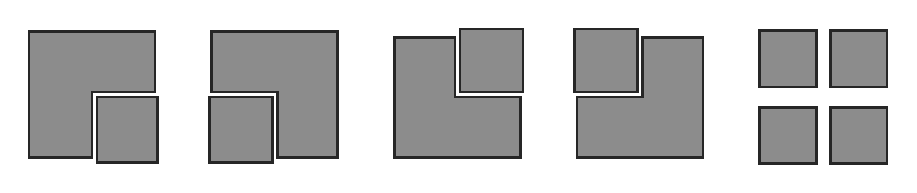
\begin{tikzpicture}[x=0.8cm,y=0.8cm,p/.style={draw=black!85,line width=1pt,fill=black!45}]
\begin{scope}[shift={(0,0)}]
\draw[p] (0,0) -- (0,2) -- (2,2) -- (2,1.04) -- (1.0,1.04) -- (1.0,0) -- cycle;
\draw[p] (1.08,-0.08) rectangle (2.04,0.96);
\end{scope}
\begin{scope}[shift={(2.9,0)}]
\draw[p] (0,2) -- (2,2) -- (2,0) -- (1.04,0) -- (1.04,1.04) -- (0,1.04) -- cycle;
\draw[p] (-0.04,-0.08) rectangle (0.96,0.96);
\end{scope}
\begin{scope}[shift={(5.8,0)}]
\draw[p] (0,0) -- (0,1.9) -- (0.96,1.9) -- (0.96,0.96) -- (2,0.96) -- (2,0) -- cycle;
\draw[p] (1.04,1.04) rectangle (2.04,2.04);
\end{scope}
\begin{scope}[shift={(8.7,0)}]
\draw[p] (0,0) -- (0,0.96) -- (1.04,0.96) -- (1.04,1.9) -- (2,1.9) -- (2,0) -- cycle;
\draw[p] (-0.04,1.04) rectangle (0.96,2.04);
\end{scope}
\begin{scope}[shift={(11.6,0)}]
\draw[p] (0,1.12) rectangle (0.9,2.02);
\draw[p] (1.12,1.12) rectangle (2.02,2.02);
\draw[p] (0,-0.1) rectangle (0.9,0.8);
\draw[p] (1.12,-0.1) rectangle (2.02,0.8);
\end{scope}
\end{tikzpicture}
\end{center}
\end{pastexam}

\begin{pastsoln}
答案：(a) $d(3) = 11$；(b) $a = 1$，$b = 4$，$c = 2$，即 $d(m) = d(m-1) + 4\,d(m-2) + 2\,d(m-3)$。

L 形是 $2 \times 2$ 的方塊少一格，所以一定剛好落在相鄰的兩行裡，有四種方向。 寫遞迴式的方法和資結書
第~2.5.5~節的鋪地磚一樣：看最左邊那一行（第 $1$ 行）是怎麼被蓋住的，把所有情形分成互不重疊的幾類，每一類
剩下的部分又是一個比較短的 $2 \times k$ 方塊。

\textbf{分類。} 設 $m \ge 3$。
\begin{enumerate}[label=(\arabic*)]
\item 第 $1$ 行的兩格都是小方塊：剩下 $2 \times (m-1)$，$d(m-1)$ 種。
\item 一個 L 蓋住第 $1$ 行的\textbf{一格}：L 落在第 $1$、$2$ 行，又只用第 $1$ 行的一格，就一定蓋滿第 $2$ 行
兩格；第 $1$ 行剩下的那一格旁邊都被佔了，只能放小方塊。 L 有 $2$ 種方向（缺上角或缺下角），剩下
$2 \times (m-2)$，共 $2\,d(m-2)$ 種。
\item 一個 L 蓋住第 $1$ 行的\textbf{兩格}和第 $2$ 行的一格（$2$ 種方向）。 第 $2$ 行剩下的那一格：
  \begin{itemize}
  \item 放小方塊：剩下 $2 \times (m-2)$，$d(m-2)$ 種；
  \item 被另一個 L 蓋住：這個 L 不能用第 $1$ 行，只能落在第 $2$、$3$ 行；第 $2$ 行只剩一格，所以它蓋住那一格
  和第 $3$ 行兩格。 兩個 L 剛好拼成 $2 \times 3$，剩下 $2 \times (m-3)$，$d(m-3)$ 種。
  \end{itemize}
  共 $2\,[d(m-2) + d(m-3)]$ 種。
\end{enumerate}
三類涵蓋了第 $1$ 行所有可能的蓋法，而且互不重疊，所以
\[
d(m) = d(m-1) + 2\,d(m-2) + 2\,[d(m-2) + d(m-3)] = d(m-1) + 4\,d(m-2) + 2\,d(m-3).
\]
$m = 3$ 時第 (3) 類的「兩個 L 拼成 $2 \times 3$」剩下寬 $0$ 的方塊，算 $d(0) = 1$ 種，正是題目假設
$d(0) = 1$ 的用意。 （用 $m = 2$ 代入、把 $d(-1)$ 當 $0$，得 $1 + 4 = 5$，和題目的 $d(2)$ 相符。）

兩個 L 拼成 $2 \times 3$ 的兩種方式：
\begin{center}
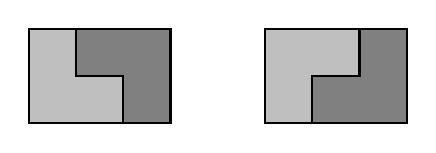
\begin{tikzpicture}[x=0.6cm,y=0.6cm,p/.style={draw=black,thick,fill=black!25}]
\draw[p] (0,0) -- (2,0) -- (2,1) -- (1,1) -- (1,2) -- (0,2) -- cycle;
\draw[p,fill=black!50] (1,1) -- (1,2) -- (3,2) -- (3,0) -- (2,0) -- (2,1) -- cycle;
\begin{scope}[shift={(5,0)}]
\draw[p] (0,0) -- (1,0) -- (1,1) -- (2,1) -- (2,2) -- (0,2) -- cycle;
\draw[p,fill=black!50] (1,0) -- (3,0) -- (3,2) -- (2,2) -- (2,1) -- (1,1) -- cycle;
\end{scope}
\end{tikzpicture}
\end{center}

\textbf{(a)} $d(3) = d(2) + 4\,d(1) + 2\,d(0) = 5 + 4 + 2 = 11$。 分開數：第 (1) 類 $d(2) = 5$；第 (2) 類
$2 \times d(1) = 2$；第 (3) 類放小方塊 $2 \times d(1) = 2$、兩個 L 拼成 $2 \times 3$ 有 $2$ 種，合計 $11$。

\textbf{(b)} $a = 1$，$b = 4$，$c = 2$。 由遞迴式，$d(4) = 11 + 20 + 2 = 33$、$d(5) = 33 + 44 + 10 = 87$、
$d(6) = 87 + 132 + 22 = 241$。 反過來，題目的形式有三個未知數，用 $m = 4, 5, 6$ 三個等式
\[
11a + 5b + c = 33, \qquad 33a + 11b + 5c = 87, \qquad 87a + 33b + 11c = 241
\]
解出的也只有 $(a, b, c) = (1, 4, 2)$ 這一組，所以答案唯一。
\end{pastsoln}
